%\documentclass[landscape]{article}
\documentclass[portrait]{article}
\usepackage[usenames]{color}

\usepackage{pgf}
\usepackage{tikz}

\usepackage{graphicx}

%\usepackage[brazil]{babel}
\usepackage[latin1]{inputenc}
\usepackage[T1]{fontenc}
\usepackage[all]{xy}

\usepackage {vmargin}           % para setar formato da página + facilmente

% Dimensões a ocupar na página (package Vmargin)
\setpapersize [portrait]{A4}
\setmarginsrb {25mm} % margem esquerda
              {25mm} % margem topo
              {20mm} % margem direita
              {20mm} % margem pé
              {2ex}  % altura do espaço para cabeçalho
              {2ex}  % espaço entre fim do cabeçalho e início do texto
              {2ex}  % altura do espaço para rodapé
              {2ex}  % espaço entre fim do texto e fim do rodapé

\usetikzlibrary{arrows,automata}
%\usetikzlibrary{positioning}
%\usetikzlibrary{arrows,decorations.pathmorphing,backgrounds,positioning,fit}
\usetikzlibrary{positioning,shapes,shadows,arrows}

%\definecolor{Peach}{rgb}{0,0.08,0.45}
\definecolor{Peach}{cmyk}{0,0.50,0.70,0}

\tikzset{
    state/.style={
           rectangle,
           fill = Peach!10,
           rounded corners,
%           draw = blue!50!black,
           very thick,
           minimum height = 2em,
           inner sep = 2pt,
           text centered,
           drop shadow,
           },
}
\tikzstyle{myarrow}=[->, >=open triangle 90, thick]

\begin{document}

\input ReachableDefinitions.tex
\clearpage

\input LiveVariable.tex
\clearpage

\input AvailableExpressions.tex
\clearpage

\input AnticipableExpressions.tex
\clearpage

\input PartiallyAvailableExpressions.tex
\clearpage

\input DeadVariable.tex
\clearpage

\input DefinitionsForCopyPropagation.tex
\clearpage

\input PartialRedundancy1.tex
\clearpage

\input ConstantPropagation.tex
\clearpage


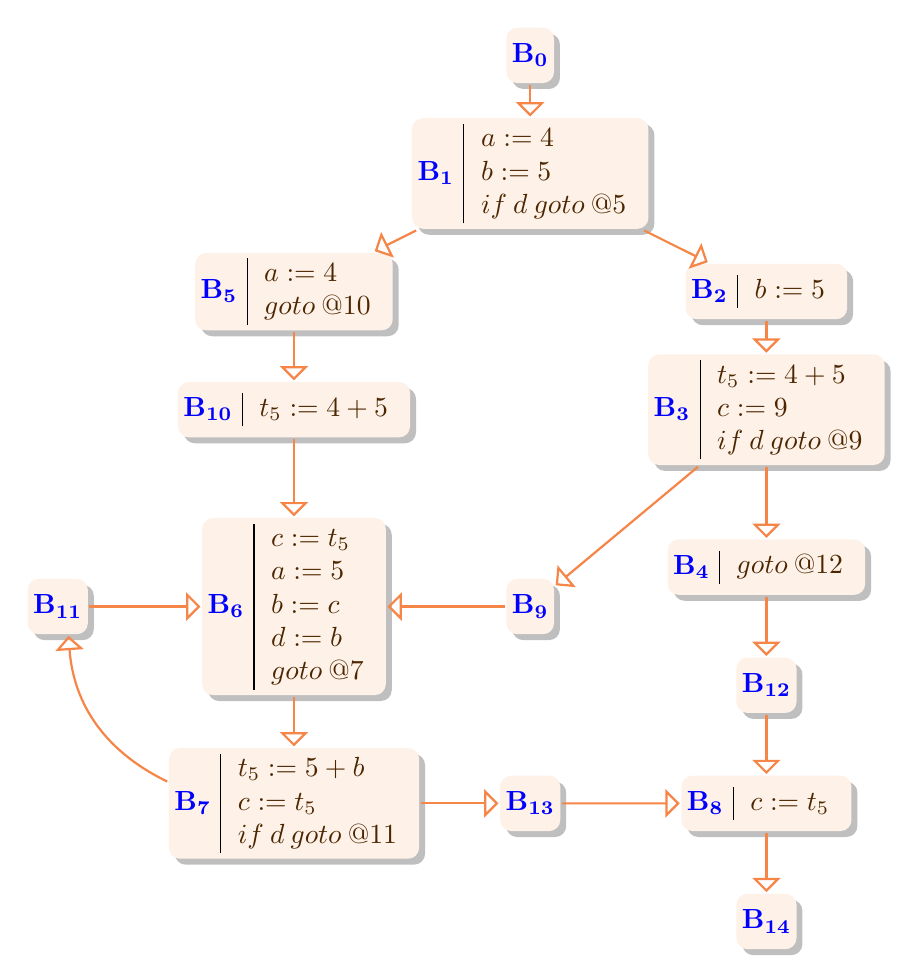
\begin{tikzpicture}[->,>=stealth']

 \node[state] (B0)
 {%
 \textcolor{blue}{\txt{$\mathbf{B_{0}}$}}
 };

\node[state,
  below of=B0,
  node distance=1.5cm,
  anchor=center] (B1)
 {%
 \textcolor{blue}{$\mathbf{B_{1}}$}
 \begin{tabular}{|l}
 {\color{orange!30!black}$a:=4$}\\
 {\color{orange!30!black}$b:=5$}\\
 {\color{orange!30!black}$if\:d\:goto\:@5$}
 \end{tabular}
 };

\node[
  right of=B1,
  node distance=3cm,
  anchor=center] (B1R)
 {};%
\node[
  left of=B1,
  node distance=3cm,
  anchor=center] (B1L)
 {};%

\node[state,
  below of=B1L,
  node distance=1.5cm,
  anchor=center] (B5)
 {%
 \textcolor{blue}{$\mathbf{B_{5}}$}
 \begin{tabular}{|l}
 {\color{orange!30!black}$a:=4$}\\
 {\color{orange!30!black}$goto\:@10$}
 \end{tabular}
 };

\node[state,
  below of=B1R,
  node distance=1.5cm,
  anchor=center] (B2)
 {%
 \textcolor{blue}{$\mathbf{B_{2}}$}
 \begin{tabular}{|l}
 {\color{orange!30!black}$b:=5$}
 \end{tabular}
 };

\node[state,
  below of=B5,
  node distance=1.5cm,
  anchor=center] (B10)
 {%
 \textcolor{blue}{$\mathbf{B_{10}}$}
 \begin{tabular}{|l}
 {\color{orange!30!black}$t_{5}:=4+5$}
 \end{tabular}
 };

\node[state,
  below of=B2,
  node distance=1.5cm,
  anchor=center] (B3)
 {%
 \textcolor{blue}{$\mathbf{B_{3}}$}
 \begin{tabular}{|l}
 {\color{orange!30!black}$t_{5}:=4+5$}\\
 {\color{orange!30!black}$c:=9$}\\
 {\color{orange!30!black}$if\:d\:goto\:@9$}
 \end{tabular}
 };

\node[state,
  below of=B10,
  node distance=2.5cm,
  anchor=center] (B6)
 {%
 \textcolor{blue}{$\mathbf{B_{6}}$}
 \begin{tabular}{|l}
 {\color{orange!30!black}$c:=t_{5}$}\\
 {\color{orange!30!black}$a:=5$}\\
 {\color{orange!30!black}$b:=c$}\\
 {\color{orange!30!black}$d:=b$}\\
 {\color{orange!30!black}$goto\:@7$}
 \end{tabular}
 };

\node[state,
  left of=B6,
  node distance=3cm,
  anchor=center] (B11)
 {%
 \textcolor{blue}{$\mathbf{B_{11}}$}
 };

\node[state,
  right of=B6,
  node distance=3cm,
  anchor=center] (B9)
 {%
 \textcolor{blue}{$\mathbf{B_{9}}$}
 };

\node[state,
  below of=B3,
  node distance=2cm,
  anchor=center] (B4)
 {%
 \textcolor{blue}{$\mathbf{B_{4}}$}
 \begin{tabular}{|l}
 {\color{orange!30!black}$goto\:@12$}
 \end{tabular}
 };

\node[state,
  below of=B4,
  node distance=1.5cm,
  anchor=center] (B12)
 {%
 \textcolor{blue}{$\mathbf{B_{12}}$}
 };

\node[state,
  below of=B12,
  node distance=1.5cm,
  anchor=center] (B8)
 {%
 \textcolor{blue}{$\mathbf{B_{8}}$}
 \begin{tabular}{|l}
 {\color{orange!30!black}$c:=t_{5}$}
 \end{tabular}
 };

\node[state,
  below of=B8,
  node distance=1.5cm,
  anchor=center] (B14)
 {%
 \textcolor{blue}{$\mathbf{B_{14}}$}
 };

\node[state,
  below of=B6,
  node distance=2.5cm,
  anchor=center] (B7)
 {%
 \textcolor{blue}{$\mathbf{B_{7}}$}
 \begin{tabular}{|l}
 {\color{orange!30!black}$t_{5}:=5+b$}\\
 {\color{orange!30!black}$c:=t_{5}$}\\
 {\color{orange!30!black}$if\:d\:goto\:@11$}
 \end{tabular}
 };

\node[state,
  right of=B7,
  node distance=3cm,
  anchor=center] (B13)
 {%
 \textcolor{blue}{$\mathbf{B_{13}}$}
 };

 \path (B0)     edge[color = Peach, myarrow] (B1)
 (B1)           edge[color = Peach, myarrow] (B2)
                edge[color = Peach, myarrow] (B5)
 (B2)           edge[color = Peach, myarrow] (B3)
 (B3)           edge[color = Peach, myarrow] (B4)
                edge[color = Peach, myarrow] (B9)
 (B4)           edge[color = Peach, myarrow] (B12)
 (B12)          edge[color = Peach, myarrow] (B8)
 (B8)           edge[color = Peach, myarrow] (B14)
 (B5)           edge[color = Peach, myarrow] (B10)
 (B10)          edge[color = Peach, myarrow] (B6)
 (B6)           edge[color = Peach, myarrow] (B7)
 (B11)          edge[color = Peach, myarrow] (B6)
 (B9)           edge[color = Peach, myarrow] (B6)
 (B7)           edge[color = Peach, myarrow] (B13)
 (B13)          edge[color = Peach, myarrow] (B8)
 (B7)           edge[color = Peach, myarrow, bend left=30] (B11)
;

\end{tikzpicture}


\begin{scriptsize}
\xy(0, 0)
	*++{\txt{$\mathbf{B_{0}}$\\}}*\frm{-,}="B0";
(0, -15)
	*++{\txt{$\mathbf{B_{1}}$\\$a:=4$\\$b:=5$\\$if\:d\:goto\:@5$\\}}*\frm{-,}="B1";
(25, -30)
	*++{\txt{$\mathbf{B_{2}}$\\$b:=5$\\}}*\frm{-,}="B2";
(25, -45)
	 *++{\txt{$\mathbf{B_{3}}$\\$t_{5}:=4+5$\\$c:=9$\\$if\:d\:goto\:@9$\\}}*\frm{-,}="B3";
(25, -60)
	*++{\txt{$\mathbf{B_{4}}$\\$goto\:@12$\\}}*\frm{-,}="B4";
(-25, -30)
	*++{\txt{$\mathbf{B_{5}}$\\$a:=4$\\$goto\:@10$\\}}*\frm{-,}="B5";
(-25, -65)
	 *++{\txt{$\mathbf{B_{6}}$\\$c:=t_{5}$\\$a:=5$\\$b:=c$\\$d:=b$\\$goto\:@7$\\}}*\frm{-,}="B6";
(-25, -90)
	 *++{\txt{$\mathbf{B_{7}}$\\$t_{5}:=5+b$\\$c:=t_{5}$\\$if\:d\:goto\:@11$\\}}*\frm{-,}="B7";
(25, -90)
	*++{\txt{$\mathbf{B_{8}}$\\$c:=t_{5}$\\}}*\frm{-,}="B8";
(50, -60)
	*++{\txt{$\mathbf{B_{9}}$\\}}*\frm{-,}="B9";
(-25, -45)
	*++{\txt{$\mathbf{B_{10}}$\\$t_{5}:=4+5$\\}}*\frm{-,}="B10";
(-50, -90)
	*++{\txt{$\mathbf{B_{11}}$\\}}*\frm{-,}="B11";
(25, -75)
	*++{\txt{$\mathbf{B_{12}}$\\}}*\frm{-,}="B12";
(0, -90)
	*++{\txt{$\mathbf{B_{13}}$\\}}*\frm{-,}="B13";
(25, -105)
	*++{\txt{$\mathbf{B_{14}}$\\}}*\frm{-,}="B14";
"B0";"B1" **@{.} ?> *{\dir{>}};
"B1";"B5" **@{.} ?> *{\dir{>}};
"B1";"B2" **@{.} ?> *{\dir{>}};
"B2";"B3" **@{.} ?> *{\dir{>}};
"B3";"B4" **@{.} ?> *{\dir{>}};
"B3";"B9" **@{.} ?> *{\dir{>}};
"B4";"B12" **@{.} ?> *{\dir{>}};
"B5";"B10" **@{.} ?> *{\dir{>}};
"B6";"B7" **@{.} ?> *{\dir{>}};
"B7";"B11" **@{.} ?> *{\dir{>}};
"B7";"B13" **@{.} ?> *{\dir{>}};
"B8";"B14" **@{.} ?> *{\dir{>}};
"B9";"B6" **@{.} ?> *{\dir{>}};
"B10";"B6" **@{.} ?> *{\dir{>}};
"B11";"B6" **@{.} ?> *{\dir{>}};
"B12";"B8" **@{.} ?> *{\dir{>}};
"B13";"B8" **@{.} ?> *{\dir{>}};
\endxy
\end{scriptsize}
\end{document}

